% Every Latex document starts with a documentclass command
\documentclass[a4paper, 11pt]{article}

% Load some packages
\usepackage{graphicx} % This allows you to put figures in
\usepackage{natbib}   % This allows for relatively pain-free reference lists
\usepackage[left=2cm,top=3cm,right=2cm]{geometry} % The way I like the margins
\usepackage{framed}

\newcommand{\dnest}{{\tt DNest4}}

% This helps with figure placement
\renewcommand{\topfraction}{0.85}
\renewcommand{\textfraction}{0.1}
\parindent=0cm

% Set values so you can have a title
\title{\dnest~Manual}
\author{Brendon J. Brewer}
\date{\today}

% Document starts here
\begin{document}

% Actually put the title in
\maketitle

\section{Introduction}

\dnest~is a multi-threaded C++ implementation of Diffusive Nested Sampling
(DNS), a powerful Markov Chain Monte Carlo (MCMC) algorithm that is mainly
useful for solving Bayesian Inference problems.
\dnest~is free software, released under the terms of the MIT licence.
For information about how the
algorithm works, please see the Diffusive Nested Sampling paper,
available from the following URL:\\

\begin{center}
{\tt http://arxiv.org/abs/0912.238}\\
\end{center}

If you find \dnest~useful in a research project,
please feel free to cite the paper.
Throughout this manual I will assume that you have read the paper and have a
reasonable understanding of how the algorithm works, as well as some
understanding of general Nested Sampling concepts.\\

\section{Installation}
Please note that I have only ever compiled \dnest~on GNU/Linux,
using the GNU C++ compiler ({\tt g++}). However, I expect it to be
straightforward to compile it on any other Unix-like operating system such as Mac
OS X or FreeBSD. It should be possible, albeit probably more tricky,
to compile \dnest~in Microsoft Windows. If you want to try,
the MinGW compiler is
probably your best bet. I'd be interested to hear from anyone who
has tried this. I would also be interested to hear if anyone has
compiled \dnest~with a different compiler, such as the Intel C++
compiler.\\

\subsection{Dependencies}
One of the issues with DNest3 which inspired a new version was that many users
found it annoying to compile on different operating systems because of the
dependencies. For that reason, \dnest~now has much less dependencies.
The C++ part of the code is written in pure C++11 and does not require any
additional libraries --- you just have to have a modern C++ compiler that
supports the C++11 standard.

The Python postprocessing scripts use the Python packages
{\tt numpy} and {\tt matplotlib}. They work with both Python 2 or 3.

\subsection{Compiling}
Go into the {\tt code} directory and run {\tt make}. Everything should compile.
To
verify that the compilation was successful,
go into the {\tt Examples/SpikeSlab} directory
and see if an executable file called {\tt main} has been created. If you
execute this file, you should see a lot of output about ``levels'' and
``particles'' (see Figure~\ref{fig:output} for example output).
You will need to manually terminate this process by using
Control+C, or whatever works in your operating system. If you saw this output,
\dnest~was compiled successfully.\\

\section{Running DNest}
As part of the compilation process, several examples will have been compiled.
There is one executable file for each example: \dnest~does not have a global
executable. The
following discussion will involve running the ``SpikeSlab'' example, which is
the example used in the paper.\\

To run the SpikeSlab example, go into the {\tt Examples/Spikeslab}
directory and execute {\tt main}. You should see some output that looks like
that shown in Figure~\ref{fig:output}.
Note that you must terminate the process manually by pressing Ctrl+C
or in another way. If you do not terminate the process yourself, it will run
forever. There is no definite rule for how long you should run \dnest.
It depends on the difficulty of your problem, the number of posterior samples you
want, and the accuracy you want for the marginal likelihood.\\

\begin{figure}[h!]
\begin{framed}
\begin{verbatim}
$ ./main
# Using 1 thread.
# Target compression factor between levels = 2.7182818284590451
# Seeding random number generators. First seed = 1452723978.
# Generating 1 particle from the prior...done.
# Creating level 1 with log likelihood = -44.1995.
# Creating level 2 with log likelihood = -32.1028.
# Creating level 3 with log likelihood = -25.5476.
# Creating level 4 with log likelihood = -19.911.
# Creating level 5 with log likelihood = -15.5224.
# Creating level 6 with log likelihood = -11.0712.
# Creating level 7 with log likelihood = -6.9397.
# Creating level 8 with log likelihood = -3.30518.
# Creating level 9 with log likelihood = 0.522437.
\end{verbatim}
\end{framed}
\caption{\it An example of \dnest~output that is shown on the screen. More
detailed information is saved to the three output files
{\tt sample.txt}, {\tt sample\_info.txt}, and {\tt levels.txt}.
\label{fig:output}}
\end{figure}

The executable {\tt main} is responsible for the exploration part of the
DNS algorithm (i.e. running the MCMC chain, building
levels, and then exploring all the levels). It creates three output text files,
{\tt sample.txt}, {\tt sample\_info.txt}, and {\tt levels.txt}.\\

The first output
file, {\tt sample.txt}, contains a sampling of parameter values that
represents the {\it mixture of constrained priors} (the target distribution
used in DNS), {\bf not} the
posterior distribution. Each line of {\tt sample.txt} represents a point in
parameter space. In the SpikeSlab example, there are 20 parameters, so there
will be 20 columns in {\tt sample.txt}.
Each time a point is saved to {\tt sample.txt}, \dnest~prints
the message ``Saving a particle to disk. N = ...''.\\

The second output file, {\tt sample\_info.txt}, should have the same number of
rows as {\tt sample.txt}, because it contains metadata about the samples in
{\tt sample.txt}. The first
column is the index $j$, which tells us which ``level'' the particle was in
when it was saved. Level 0 represents the prior, and higher levels represent
more constrained versions of the prior.
The second column is the log-likelihood value, and the third column is
the likelihood ``tiebreaker'', which allows Nested Sampling to work when
there is a region in parameter space with nonzero prior probability where the
likelihood is constant. The final column tells us which thread the particle
belonged to: when you use \dnest~in multithreaded mode, each thread
is responsible for evolving one or more walkers.\\

The third output file, {\tt levels.txt}, contains information about the levels
that were built during the run. The first column has estimates of the $\log(X)$
values of the levels, i.e. how compressed they are relative to the prior, in
units of nats. The second column contains the log likelihoods of the levels.
The first level, with a $\log(X)$ value of 0 and a log likelihood of
$-10^{300}$ (basically ``minus infinity''), is simply the prior. The third
column has the ``tiebreaker'' values for the levels, which again are not
particularly useful unless your problem has likelihood plateaus. The fourth
and fifth columns are the number of accepted proposals and the total number
of proposals that have occurred within each level, which are useful for
monitoring the Metropolis acceptance ratio as a function of level.
The final two columns, called ``exceeds'', and ``visits'', are used to refine
the estimates of the level compressions (and hence the $\log(X)$ values of
the levels in column 1), as discussed in Section 3 of the
paper. The visits column counts the number of times a level (level $j$, say)
has been visited, but only starts counting after the next level ($j+1$) has been created. The exceeds column counts the number of times a particle that was
in level $j$ had a likelihood that exceeded that of level $j+1$.
\\

\section{Postprocessing with showresults.py}
After {\tt main} has been running for
a while, you should run the postprocessing script
by executing {\tt python showresults.py}. This script loads the output files,
plots some graphs, and creates two new output files, {\tt weights.txt} and
{\tt posterior\_samples.txt}. It also prints the current estimate of the
(log of the) marginal likelihood or evidence value (traditionally considered
the main goal of Nested Sampling), as well as the information value (the KL
divergence from the prior to the posterior).\\

The plots made by {\tt showresults.py} are very similar to the plots in
the DNS paper. The first plot shows the level of the saved particles vs.
time, the equivalent of Figure 2 in the paper. The second plot produced by
{\tt showresults.py} shows the estimated compression values of the levels,
like in Figure 3 of the paper, along with the Metropolis acceptance fraction
as a function of the level (as you would expect, this usually shows a
decreasing trend). The red horizontal line on the level compression plot is
at -1, and all of the actual compressions should be close to -1 if everything
is working well (unless you've changed the target compression from $e$ to
another value as discussed in Section~\ref{sec:commandline}).

The final plot corresponds to Figure 4 from the paper, and
shows the shape of the likelihood curve along with the posterior weights of
the saved particles.\\

The plots are useful for diagnosing the progress of your run. For example, you
want to ensure that the Metropolis acc
eptance fraction doesn't drop to near
zero. If it does, the proposal distributions might be too aggressive, or maybe
you just created too many levels (and the high level distributions are just
extremely narrow). The other key plot for diagnostics is the posterior
weights. On most problems, these will peak at some point, and begin to
come back down towards zero (See Figure~\ref{fig:fig3}).
Once this occurs, you probably have enough levels.
It is wasteful to create large amounts of levels extending well beyond the peak.
However, on problems with phase transitions more than one peak may occur.
An example of not having enough levels is given in
Figure~\ref{fig:not_enough_levels}. To change the number of levels, you
can use the OPTIONS file, described in Section~\ref{sec:options}.\\

\begin{figure}
\begin{center}
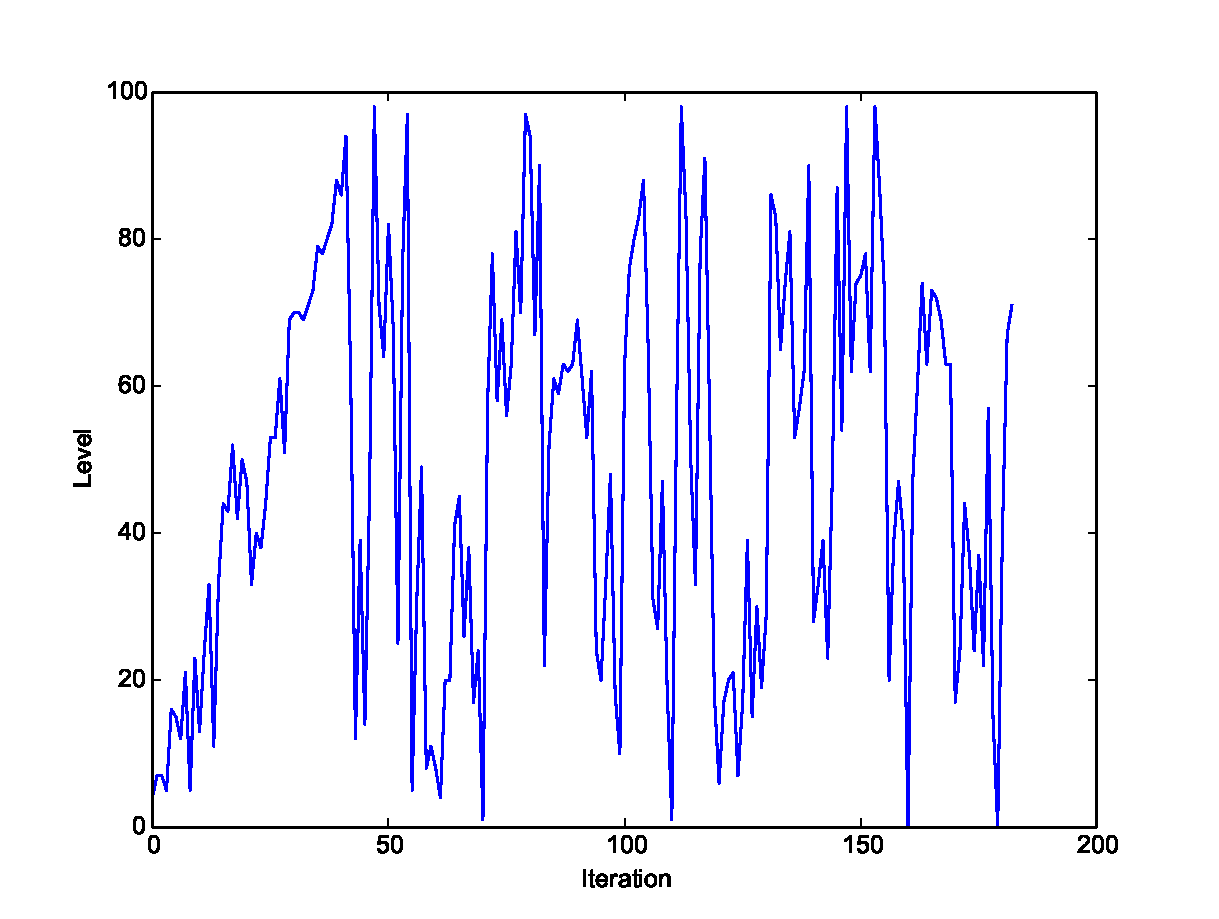
\includegraphics[scale=0.5]{fig1.pdf}
\caption{\it Level vs. Time from a \dnest~run with 100 levels.\label{fig:fig1}}
\end{center}
\end{figure}

\begin{figure}
\begin{center}
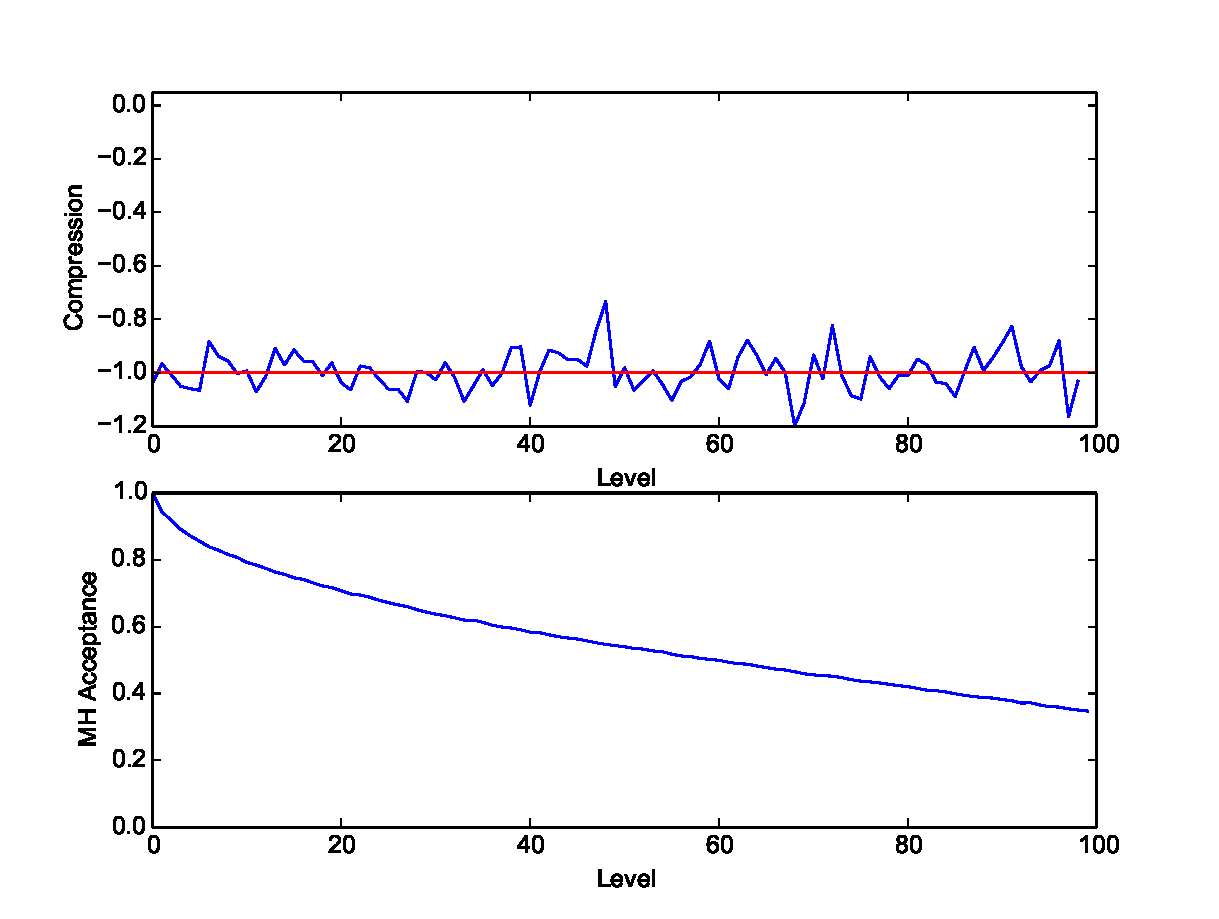
\includegraphics[scale=0.5]{fig2.pdf}
\caption{\it Top panel: Estimated compressions between adjacent levels. Ideally, these should equal -1. Bottom panel: Metropolis-Hastings acceptance ratio
as a function of level.\label{fig:fig2}}
\end{center}
\end{figure}

\begin{figure}
\begin{center}
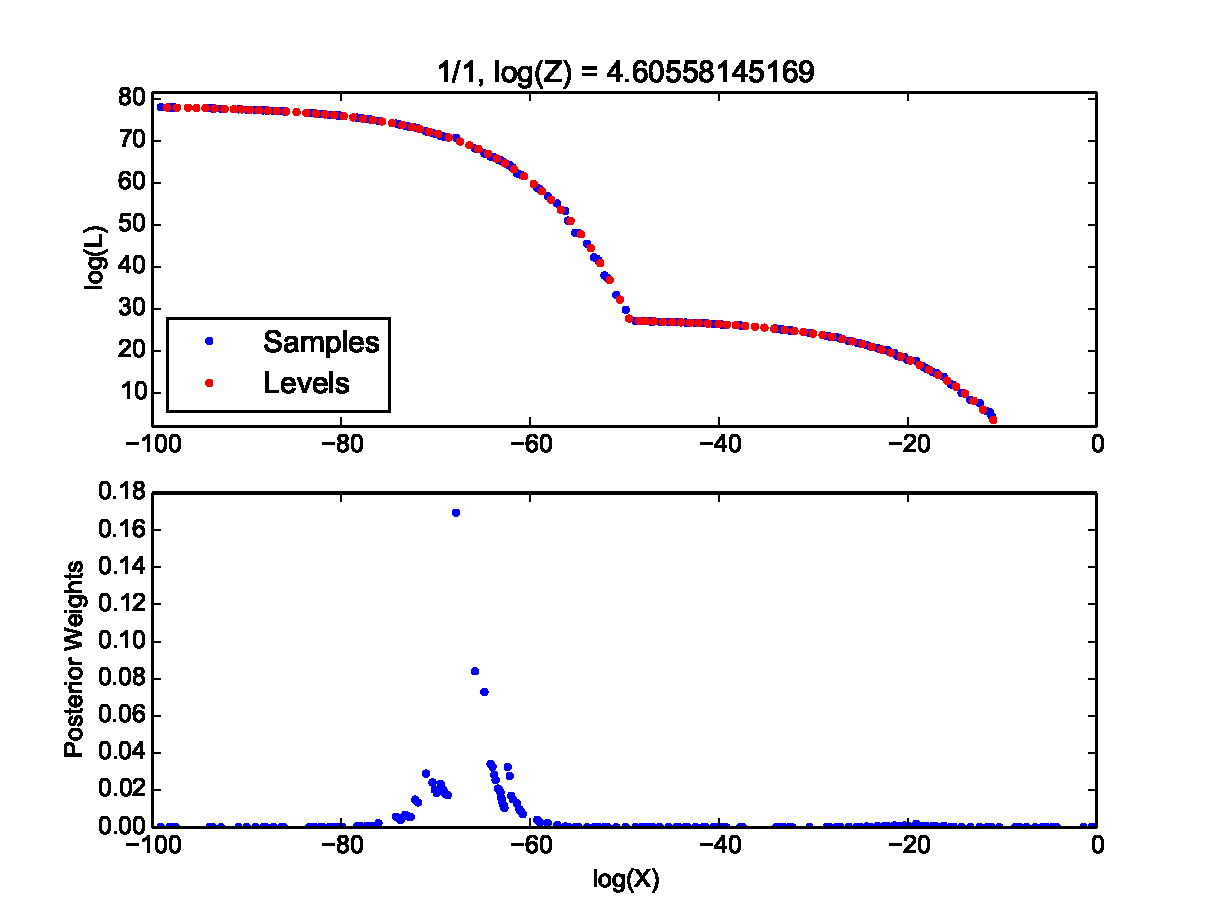
\includegraphics[scale=0.5]{fig3.pdf}
\caption{\it Top panel: Likelihood as a function of enclosed prior mass,
the standard Nested Sampling plot. Bottom panel: Posterior weights as a
function of enclosed prior mass. If this peaks at the left of the plot,
i.e. you can't see an entire peak, you need more levels.\label{fig:fig3}}
\end{center}
\end{figure}


\begin{figure}
\begin{center}
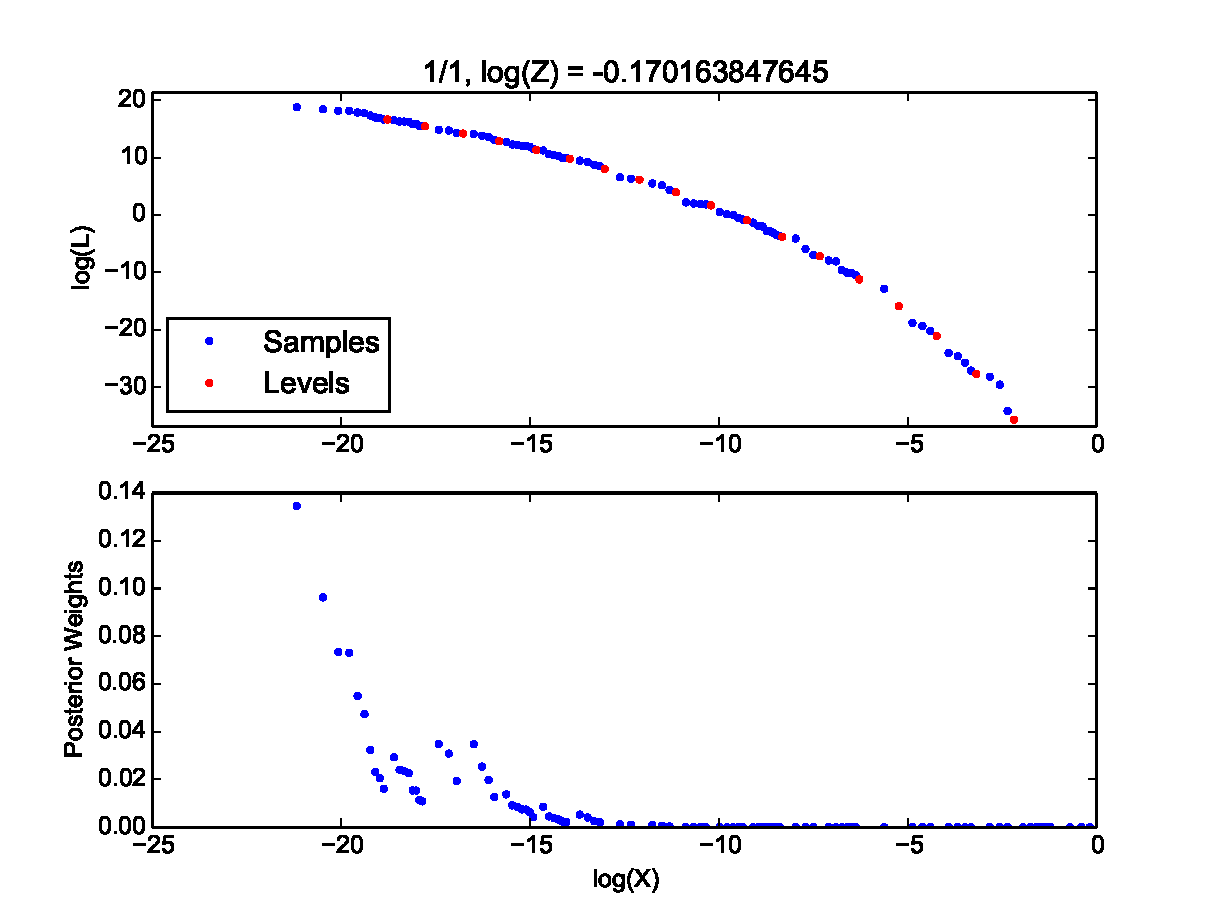
\includegraphics[scale=0.5]{not_enough_levels.pdf}
\caption{\it Top panel: Example of a DNest run where the number of levels
was too low. The posterior weights peak at the left of the plot, and these
would have continued to increase if we'd gone further.
\label{fig:not_enough_levels}}
\end{center}
\end{figure}

\section{Command line options}\label{sec:commandline}
\dnest~executables allow for several command line options. A couple of these
options are quite important, while others are much less useful.
You can view the available options by executing
{\tt ./main -h}. Here is the list:\\

\begin{figure}
\begin{framed}
\begin{verbatim}
DNest4 Command Line Options: 
-h: display this message
-o <filename>: load DNest4 options from the specified file. Default=OPTIONS
-s <seed>: seed the random number generator with the specified value.
           If unspecified, the system time is used.
-d <filename>: Load data from the specified file, if required.
-c <value>: Specify a compression value (between levels) other than e.
-t <num_threads>: run on the specified number of threads. Default=1.
\end{verbatim}
\end{framed}
\end{figure}

The most important option is the one about the number of threads. Depending on
your computer, you probably want to run \dnest~with more than one thread.
Each thread will be responsible for evolving its own walker(s), and periodically
the threads will pool their results (for example, information about the
levels). To execute \dnest~with 8 threads, simply use {\tt ./main -t 8}. You can
replace 8 with however many threads you want. I usually use 8 threads because
that's how many my computer can run simultaneously at full speed.\\

In many Monte Carlo studies, it is useful to be able to set the random number
seed, for debugging and reproducibility reasons. By default \dnest~seeds the
random number generator with the system time, and displays the value of the
seed in the output (you can see this in the example output displayed above).
If you want to set the seed to
something else, use the {\tt -s} option and specify a non-negative integer for
the seed. For example, to execute \dnest~with
8 threads and a seed of 42, use {\tt ./main -t 8 -s 42}.
When running with multiple threads, \dnest~uses a separate generator for each
thread, and ensures that they are seeded with different values.\\

\section{The OPTIONS file}\label{sec:options}
Here is an example OPTIONS file.
\begin{framed}
\begin{verbatim}
1       # Number of particles
10000   # new level interval
100000  # save interval
200     # threadSteps
100     # maximum number of levels
10      # Backtracking scale length (lambda in the paper)
10      # Strength of effect to force histogram to equal push. (beta in the paper)
0       # Maximum number of saves (0 = infinite)
\end{verbatim}
\end{framed}

The first option is the number of particles {\it per thread}. If you run
\dnest~with 8 threads, there will actually be 8 particles. For most
applications, 1 particle per thread is sufficient. If you use more particles
per thread, the same amount of CPU time will be spent evolving more particles,
so each one will not be evolved as far. On most problems, one particle per
thread is fine. I would only use more particles per thread when working on
a very hard problem where it is difficult for the particles to find the
important parts of parameter space.\\

The new level interval controls how quickly \dnest~creates new levels. In this
example, this is set to 10,000, so a new level will be created once \dnest~has
seen 10,000 likelihood values above the current top level. This is not affected by
the number of threads. It is difficult to give a sensible default for this
quantity because it depends on the complexity of the problem and how good
the Metropolis proposals are. However, 10,000
will work for many problems (I rarely use anything less than 10,000 or greater
than 300,000). Higher values are slower, but more fail-safe.\\

The save interval controls how often \dnest~writes a model to the output
files: this is what is usually called ``thinning''. Saving more frequently
(i.e. a smaller save interval) is usually better, although it depends on your
problem. If your models have a lot of parameters {\tt sample.txt} can get
very big and take forever to process using {\tt showresults.py}. A default
suggestion that is usually okay is to make the save interval the same as the
new level interval.\\

The option ``threadSteps'' controls how frequently the separate threads pool
their information about the levels. I usually use 100 or 200. If
(threadSteps) $\times$ (number of threads) is not much smaller than
saveInterval or newLevelInterval, the latter won't be what you expect, because
\dnest~only creates levels or saves particles when the threads are pooling
information.\\

\section{Implementing models}
\dnest~currently includes three example models: SpikeSlab, StraightLine,
RJObject\_SineWaves, and RJObject\_GalaxyField.
It also contains an empty Template example which you can use
to implement your own models.\\

To use \dnest~on a particular problem, you need to implement a C++ class
which describes the features of the model (e.g. what the parameters are,
what the prior is, and what the likelihood is). Specifically, an object
(instance) of your class represents a point in the parameter space of your
problem. The class must define several member functions which can be
applied to any object. The first is {\tt from\_prior(DNest4::RNG\&)},
which when called,
initialises the object with parameter values from the prior distribution
(the argument is a random number generator object, passed by reference).
The second important member function is {\tt perturb(DNest4::RNG\&)}, which is used to propose
a change to the parameters, as in the basic Metropolis algorithm. The third
is {\tt log\_likelihood()}, which returns (as you might expect)
the log of the likelihood function evaluated at the object's current position. Next,
we have the {\tt print(std::ostream\&)} member function which defines how the model
parameters are to be written to the file (i.e. which parameters are to be
printed, and in what order). Finally, there is {\tt description()},
which allows you to put a header at the top of the output files with information
about what is in each column. To demonstrate how these member functions work, we'll go
through the code for {\tt SpikeSlab}.\\

In the SpikeSlab directory,
the relevant class is the {\tt SpikeSlab} class which is defined in the files
{\tt SpikeSlab.h} and {\tt SpikeSlab.cpp}. If you open {\tt SpikeSlab.h},
you'll see that the class has only one variable, which is a C++ valarray called
{\tt params}. This contains the 20 parameter values.\\

\begin{figure}
\begin{framed}
\begin{verbatim}
class SpikeSlab
{
    private:
        std::valarray<double> params;
\end{verbatim}
\end{framed}
\end{figure}

It's up to you whether you want to have a single vector or valarray of parameters, like
in {\tt SpikeSlab}, or if you want to name all your parameters with names that
make sense to you.\\

In {\tt SpikeSlab.cpp}, all of the member function of the {\tt SpikeSlab} class
are defined. First, we have the {\it constructor}, which defines what happens
when we create an object of class {\tt SpikeSlab}:\\

\begin{framed}
\begin{verbatim}
SpikeSlab::SpikeSlab()
:params(20)
{

}
\end{verbatim}
\end{framed}

This constructor does nothing except specify the size of the {\tt params}
valarray, which in this example is 20. Next we have {\tt from\_prior(DNest4::RNG\&)}, the
function which generates the 20 parameters from the prior. In the SpikeSlab
example, the prior is Uniform$(-0.5, 0.5)$, so this function just has a loop
which generates each value from this distribution. Here I'm making use of
a function {\tt rng.rand()} which generates values from $U(0, 1)$ using the
random number generator called rng (which is passed in by \dnest).
The RNG class is defined in {\tt RNG.h} within \dnest, and is really just a
wrapper of C++11's random number generator, with more convenient function names.

\begin{framed}
\begin{verbatim}
void SpikeSlab::from_prior(RNG& rng)
{
    for(size_t i=0; i<params.size(); i++)
        params[i] = -0.5 + rng.rand();
}
\end{verbatim}
\end{framed}

The next important member function is {\tt perturb(DNest4::RNG\&}, which defines the Metropolis
proposals that are used to explore. Since \dnest~spends some time sampling
the prior, and some time sampling narrow distributions like the posterior,
it's a good idea to use very heavy tailed proposal distributions. In the
SpikeSlab example, the prior width is 1, so you shouldn't make moves much
bigger than that, but you don't have any real idea how narrow the posterior
distribution is until you've solved the problem. In the SpikeSlab example,
the proposal is done by choosing one of the 20 parameters to move, and making
a move according to a scale mixture of gaussians (equivalent to ``a gaussian
proposal with a random step size''). Finally, to prevent any proposals outside
the prior range, I use modulo to ensure the proposed value is between -0.5
and 0.5. The resulting proposal is:\\

\begin{framed}
\begin{verbatim}
double SpikeSlab::perturb(RNG& rng)
{
    int which = rng.rand_int(params.size());
    params[which] += pow(10., 1.5-6*rng.rand())*rng.randn();
    params[which] = mod(params[which] + 0.5, 1.) - 0.5;
    return 0.;
}
\end{verbatim}
\end{framed}

For convenience, I recently defined two useful functions {\tt randh()}
(to generate heavy tailed proposals) and
{\tt wrap(double\& value, double min, double max)} (to simplify the modulo
stuff). An equivalent version of {\tt perturb} is then:\\

\begin{framed}
\begin{verbatim}
double SpikeSlab::perturb(RNG& rng)
{
    int which = rng.rand_int(params.size());
    params[which] += rng.randh();
    wrap(params[which], -0.5, 0.5);
    return 0.;
}
\end{verbatim}
\end{framed}

The last thing we need to pay attention to in the perturb function is the
returned value. \dnest~assumes that your perturb function, if used repeatedly,
would inherently explore the prior distribution in your problem. With
a uniform prior, it's easy to ensure this using wrap, as shown above.
However, for a non-uniform prior,
it's not so easy. One way to do it is to work in a coordinate system where
the prior {\it is} uniform, and then transforming the parameter before using
it in the likelihood function. Another way is to return a nonzero value from
the {\tt perturb} function. Any value returned is added to the log of the
acceptance probability. So if you want to explore a non-uniform prior, you
can return the log of the ratio of the prior density at the proposed point
to the value at the original point. For concreteness, suppose you had a
parameter $a$ with a Uniform$(0,10)$ prior, and a parameter $b$ with a
Normal$(20, \sigma=5)$ prior. Then the {\tt perturb} member function could be implemented
like this:\newpage

\begin{framed}
\begin{verbatim}
double MyModel::perturb(RNG& rng)
{
    int which = rng.rand_int(2);
    double logH = 0.;

    if(which == 0)
    {
        a += 10*rng.randh();
        wrap(a, 0., 10.);
    }
    else
    {
        logH -= -0.5*pow((b - 20.)/5., 2);
        b += 5*rng.randh();
        logH += -0.5*pow((b - 20.)/5., 2);
    }

    return logH;
}
\end{verbatim}
\end{framed}

This proposal chooses to move either $a$ or $b$, and uses a heavy tailed
proposal distribution (scaled by the width of the prior). Since the prior for
$b$ is non-uniform, it returns the log of the ``Hastings factor'' that would
be needed to explore the normal prior.\\

When you write a new model for \dnest, I highly recommend sampling the prior
and making sure you at least get that part correct. To do this, edit OPTIONS
so the maximum number of levels is 1, and make the save interval frequent.
Then inspect {\tt sample.txt} and make plots to ensure you're sampling the
prior correctly. If you are, that's a necessary but not sufficient condition
for your {\tt perturb} function being okay (your proposals need to satisfy
detailed balance, and it's possible to have proposals that explore the prior
well but do not satisfy detailed balance. Most simple proposals do satisfy
detailed balance).\\

The {\tt log\_likelihood} member does what you'd expect: evaluates and returns
the log likelihood based on the current setting of the parameters. In the
SpikeSlab example, the likelihood is an invented mixture of two gaussians.
However, in general, your likelihood will depend on a data set. When I'm using
real data, I usually write a {\tt Data} class, an object of which represents
a data set. Since you need to access the dataset from within another class,
it's easiest to make the C++ equivalent of a ``global variable'': a single
static instance of the dataset which is accessible from everywhere. See
the StraightLine example if you want to see a Data class.\\

Finally, the {\tt print} function defines how your parameters are printed to the
{\tt sample.txt} (and subsequently {\tt posterior\_sample.txt}) files. In
SpikeSlab, {\tt print} writes all 20 parameters, separated by
spaces, to a single line of the stream ``out'' which is input to the function:\\

\begin{framed}
\begin{verbatim}
void SpikeSlab::print(std::ostream& out) const
{
    for(size_t i=0; i<params.size(); i++)
        out<<params[i]<<' ';
}
\end{verbatim}
\end{framed}

Your print function needs to output parameters on a single line, in any order
you want. These will be the order in which they'll appear in the output files
{\tt sample.txt} and {\tt posterior\_sample.txt}. As an example, for our
above hypothetical model with parameters $a$ and $b$, the print function
and the description function might look like this:

\begin{framed}
\begin{verbatim}
void MyModel::print(std::ostream& out) const
{
    out<<a<<' '<<b<<' ';
}

string MyModel::description() const
{
    return string("a, b");
}
\end{verbatim}
\end{framed}

\subsection{Compiling and running your model}
Assuming you implemented your model in the Template directory, there's not
much else for you to do. The file {\tt main.cpp} already contains all the code
you need to construct a sampler and execute it. If your model involves a data
set, you'll just need to make sure you load the dataset at the beginning
of the {\tt main()} function, before doing anything else.\\

The Makefile in the Template directory should allow you to compile your model
by issuing the command {\tt make} in a terminal. The only preparation you need
to do is add the path to your \dnest~directory to an environment variable called
DNEST4\_PATH so that the compiler knows where \dnest~is on your system.
For example, on my laptop, \dnest~is located in /home/brewer/Projects/DNest4.
So I set DNEST4\_PATH to /home/brewer/Projects.
{\bf Note: }The \#include statements in the working examples expect to find
the \dnest~header files two directories up: i.e. the working examples will only
successfully compile without modification from within the Examples directory.
However, the Template should compile from anywhere on your system provided you
have set DNEST4\_PATH correctly.

If everything worked well then after running {\tt make},
the executable {\tt main} should exist, which you can use to run
\dnest~on your model. As always, the first time you run \dnest~on a new model,
you should pay attention to the output plots and make sure everything is okay,
such as the number of levels etc.


%\subsection{Implementing a model using Julia}
%Experimental support for models implemented in Julia is provided in the
%{\tt Examples/JuliaModel} directory. To use this, follow these steps:

%\begin{enumerate}
%\item Implement your log likelihood in {\tt julia\_model.jl}, as a function
%	called {\tt log\_likelihood} that takes a {\tt Vector::Float64} as an argument
%	and returns a {\tt Float64}. You should assume that the priors for the
%	parameters are independent Uniform(0, 1) distributions. To use
%	a different prior, transform the parameters inside
%	your log likelihood function before moving them.\\
%\item You may add other functions to {\tt julia\_model.jl}, for example to load
%	a dataset to refer to in your log likelihood.\\
%\item Edit the constructor for {\tt MyModel} in {\tt MyModel.cpp} so the parameter
%	vector has the correct length for your problem. The default given value
%	is 20.\\
%\item Open the {\tt Makefile} and make sure the {\tt -L} option passed to
%	{\tt g++} points to the
%	directory on your computer where the Julia shared library (such
%	as {\tt libjulia.so}) is stored. You might also have to configure your
%	system so that it searches for libraries here at runtime, e.g.
%	by running ldconfig as root. The \dnest~library and include files should
%	also be somewhere where the compiler will find them (or you can add them
%	to the {\tt g++} calls in the {\tt Makefile} using {\tt -I} for header
%	files and {\tt -L} for libraries).\\
%\item Open {\tt main.cpp} and edit the first argument to the function
%	{\tt jl\_init\_with\_image} to be the path to the file {\tt sys.so} associated with
%	Julia on your system.\\
%\item Compile by invoking '{\tt make}'.\\
%\item Run the executable! Note: only a single thread can be used, so you might want
%	to use the {\tt OPTIONS} file to have more than one particle. Five is a
%	reasonable default.
%\end{enumerate}

\end{document}

